% This must be in the first 5 lines to tell arXiv to use pdfLaTeX, which is strongly recommended.
\pdfoutput=1
% In particular, the hyperref package requires pdfLaTeX in order to break URLs across lines.

\documentclass[11pt]{article}
% Remove the "review" option to generate the final version.
\usepackage[review]{emnlp2021}

% Standard package includes
\usepackage{times}
\usepackage{latexsym}

% For proper rendering and hyphenation of words containing Latin characters (including in bib files)
\usepackage[T1]{fontenc}
% For Vietnamese characters
% \usepackage[T5]{fontenc}
% See https://www.latex-project.org/help/documentation/encguide.pdf for other character sets

% This assumes your files are encoded as UTF8
\usepackage[utf8]{inputenc}

% This is not strictly necessary, and may be commented out,
% but it will improve the layout of the manuscript,
% and will typically save some space.
\usepackage{microtype}
\usepackage{amssymb}
\usepackage{graphicx}

% If the title and author information does not fit in the area allocated, uncomment the following
%
%\setlength\titlebox{<dim>}
%
% and set <dim> to something 5cm or larger.

\title{Meta Representation Learning for Continual Few-shot Event Detection}


\author{First Author \\
  Affiliation / Address line 1 \\
  Affiliation / Address line 2 \\
  Affiliation / Address line 3 \\
  \texttt{email@domain} \\\And
  Second Author \\
  Affiliation / Address line 1 \\
  Affiliation / Address line 2 \\
  Affiliation / Address line 3 \\
  \texttt{email@domain} \\}

\begin{document}
\maketitle\begin{abstract}
Event types are usually predefined while the ontology of event types keep expanding and changing in the real word scenarios. Continual event detection always suffers from high computation cost or catastrophic forgetting. We propose to adapt 
\end{abstract}


\section{Introduction}
\label{sec:introduction}
These instructions are for authors submitting papers to EMNLP 2021 using \LaTeX. They are not self-contained. All authors must follow the general instructions for *ACL proceedings,\footnote{\url{http://acl-org.github.io/ACLPUB/formatting.html}} as well as guidelines set forth in the EMNLP 2021 call for papers. This document contains additional instructions for the \LaTeX{} style files.

The templates include the \LaTeX{} source of this document (\texttt{emnlp2021.tex}),
the \LaTeX{} style file used to format it (\texttt{emnlp2021.sty}),
an ACL bibliography style (\texttt{acl\_natbib.bst}),
an example bibliography (\texttt{custom.bib}),
and the bibliography for the ACL Anthology (\texttt{anthology.bib}).


\section{Problem Formulation}
\label{sec:formulation}
At first, introduce some Automatic Content Extraction (ACE) terminologies to help understand the Event Detection tasks \citep{cao2020incremental}: "\textbf{Event trigger} refers to a word that most clearly expresses the occurrence of an event. \textbf{Event arguments} are participants of the event. \textbf{Event mention} refers to a phrase or sentence within which an event is described."

Because Continual Event Detection (CED) in Natural Language problem can be viewed as a kind of Continual Learning Prediction (CLP), this paper, which majorly exploits meta-learning based methods, formulate the CED problem based on the CLP problem formulation from \citet{javed2019meta}.
A Continual Event Detection (CED) in Natural Language problem consists of an endless data stream:
\[\mathcal{T} = (X_1, Y_1), (X_2, Y_2), \dots, (X_t, Y_t), \dots\]
for inputs $X_t$ (event mentions) and targets $Y_t$ (event types), from sets $\mathcal{X}$ and $\mathcal{Y}$. The random vector $Y_t$ is sampled
according to an unknown distribution $p(Y|X_t)$. We define $S_k = (X_{j+1}, Y_{j+1}), (X_{j+2}, Y_{j+2}), \dots, (X_{j+k}, Y_{j+k})$ as a trajectory of length k which is smapled randomly from the CET problem $\mathcal{T}$, and $p(S_k|\mathcal{T})$ represents a distribution over all the trajectories $S_k$.

Our goal is to learn a function $f_W,\theta$ which predict $Y_t$ for $X_t$, and minimize the loss function below for a CED problem:
\begin{equation}
    \begin{split}
    &\mathcal{L}_{C E D}(W, \theta) \stackrel{\text { def }}{=}  \mathbb{E}\left[\ell\left(f_{W, \theta}(X), Y\right)\right] \\ 
    & =\int\left[\int \ell\left(f_{W, \theta}(x), y\right) p(y \mid x) d y\right] \mu(x) d x
    \end{split}
\end{equation}
where $W$ and $\theta$ are the parameters to be updated to minimize the objective $\mathcal{L}_{C E D}$.


\section{Method}
\label{sec:method}
\section{Method}

\subsection{Meta-learning Representation Learning}
\label{sec:mlr}
Here we propose a model-agnostic meta-learning framework composed of two modules: $\phi_\theta(X)$, a deep Representation Module (RM) parametrized by $\theta$ - from $X$ to $\mathbb{R} ^ {h}$; $g_W$, an Adaption Module (AM) parameterized by $W$ - from $\mathbb{R} ^ {h}$ to $y$. The architecture of this composed module, $f_{\theta, w} = g_W(\phi_\theta(X))$ is shown in figure \ref{img:1} . We follow a similar setup as **: $\theta$ is a meta-parameter that is learned by minimizing the meta-objective and is only updated during meta-training. Then, $W$ is learned from trajectory using fully online stream data in a single pass.

\begin{figure*}[ht]
\centering
    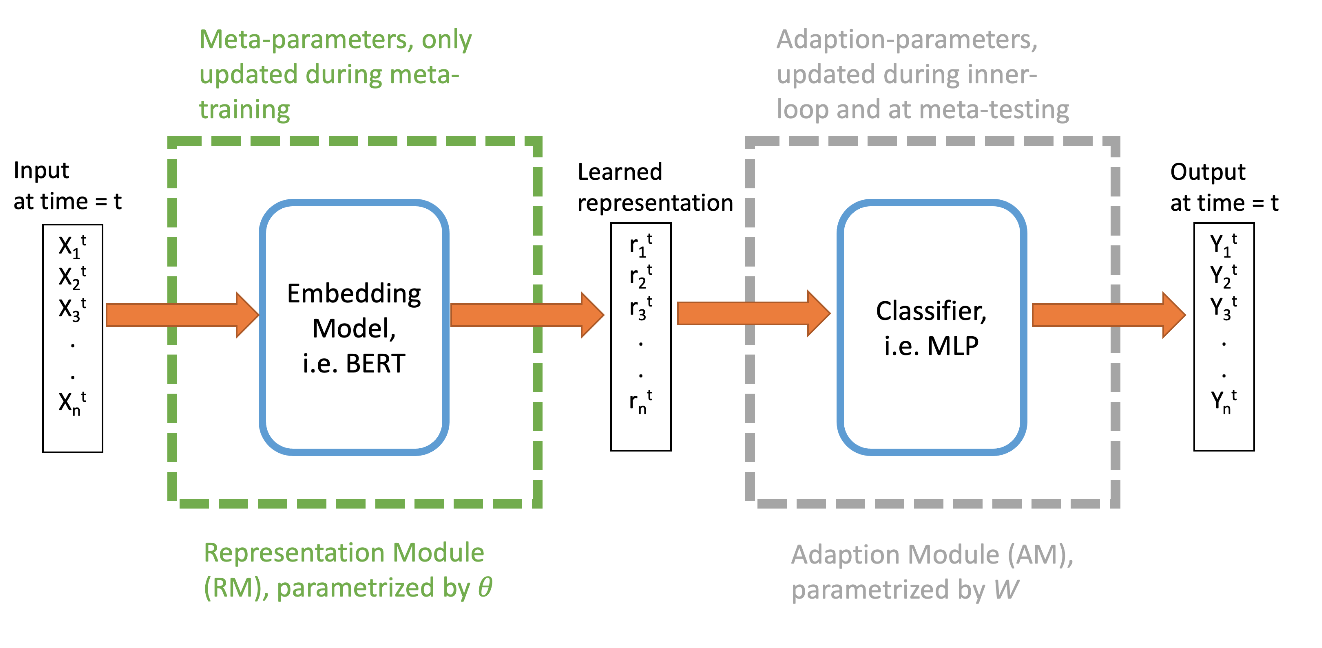
\includegraphics[scale=0.6]{imgs/framework.jpg}
    \caption{Our proposed framework composed of two modules: Representation Module and Adaption Module}
    \label{img:1}
\end{figure*}

We adapted Online-aware Meta-learning (OML) as our meta-objective for updating $\theta$ in Representation Module. OML objective could help maximize fast adaption for training the Representation Module as well as minimizing interference and is defined as:
\begin{equation}
    \begin{aligned}
       \min_{W, \theta} \sum_{\mathcal{T}_i \sim p(\mathcal{T})} \mathrm{OML}(W, \theta) \\
       = \sum_{\mathcal{T}_i \sim p(\mathcal{T})} \sum_{\mathcal{S}_k ^ j \sim p(\mathcal{S}_k | \mathcal{T}_i)} [\mathcal{L}_i (U(W, \theta, \mathcal{S}_k ^ j)]
   \end{aligned}
\end{equation}

where $p(\mathcal{T})$ is the assumed distribution for this continual learning problem; $\mathcal{S}_k ^ j = (X_{j+1}^i, Y_{j+1}^i), ..., (X_{j+k}^i, Y_{j+k}^i)$, a random trajectory of length $k$ sampled from $p(\mathcal{T})$. And $U(W, \theta, \mathcal{S}_k ^ j) = (W_{t+k}, \theta)$ is an updated function where $W_{t+k}$ is the weights of Adaption Module after $k$ steps of parameter updates, where the $jth$ update step in $U$ is on parameters $(W_{t+j-1}, \theta)$ with samples $(X_{j+t}^i, Y_{j+t}^i)$. We can see that OML only uses one data point from the trajectory, $\mathcal{S}_k ^ j$, which would help the model overcome the common problems of catastrophic forgetting in continual learning. 

Here, we use BERT * as our Representation Module due to its strong linguistic representation learning ability and a one-layer fully-connected network as our Adaption Module. 

\subsection{Meta-Training and Meta-Testing Workflow}
As stated in section \ref{sec:mlr}, we update both Representation Module and Adaption Module only in meta-training phase, which is composed of four steps as shown in figure 2 below: 
1. Suppose there is a data stream $\mathcal{T} = (X_0, Y_0), (X_1, Y_1), (X_2, Y_2), ..., (X_n, Y_n)$, we randomly sample a trajectory $\mathcal{S}_{support}$ of length $k$ as our support set for inner updates and another trajectory $\mathcal{S}_{query}$ for evaluation. \\
2. We use $\mathcal{S}_{support}$ to do $k$ continual gradient updates on Adaption Module following OML training objective, from  $W_1$ to $W_2$, ..., to $W_k$. \\
3. Next, we run evaluation of $\mathcal{S}_{query}$ using the updated network to obtain a loss; this loss would be back-propagated with respect to the initial parameters, $\theta$ of RM and $W_1$ of AM. \\
4. Finally we update both of RM and AM, from  $\theta$, $W_1$ to $\theta'$, $W_1'$.

For meta-testing, we would freeze Representation Module and simply update the Adaption Module following the step 2 in meta-training using the support set. Then we make predictions on query set with the updated Adaption Module and freeze Representation Module.
\begin{figure*}[ht]
\centering
    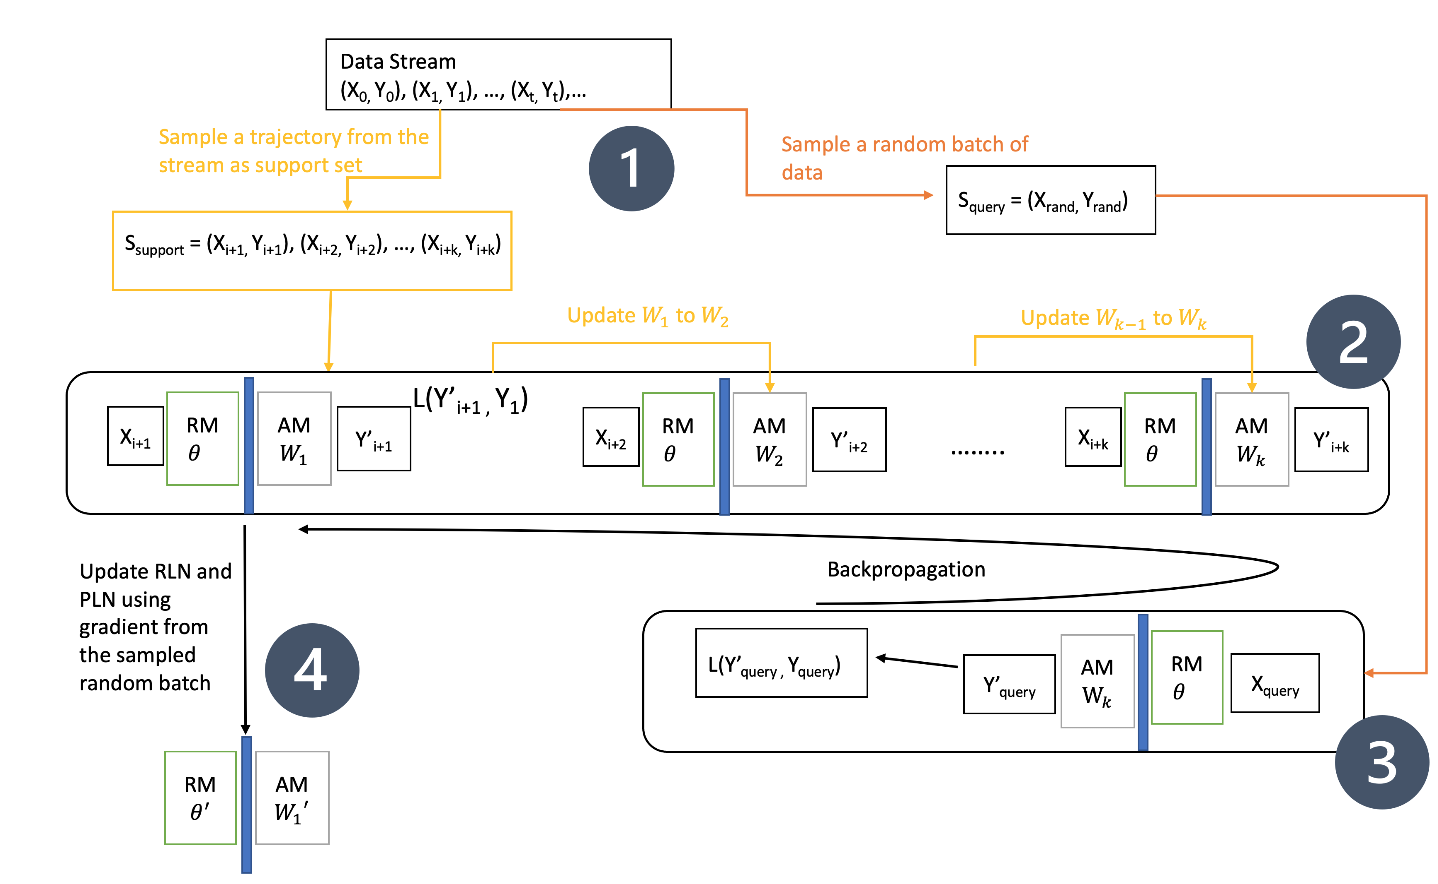
\includegraphics[scale=0.6]{imgs/meta-training.png}
    \caption{Meta-training Workflow}
    \label{img:2}
\end{figure*}



\section{Experiment }
\label{sec:experiment}


%   \begin{figure*}[ht]
%     \centering
%      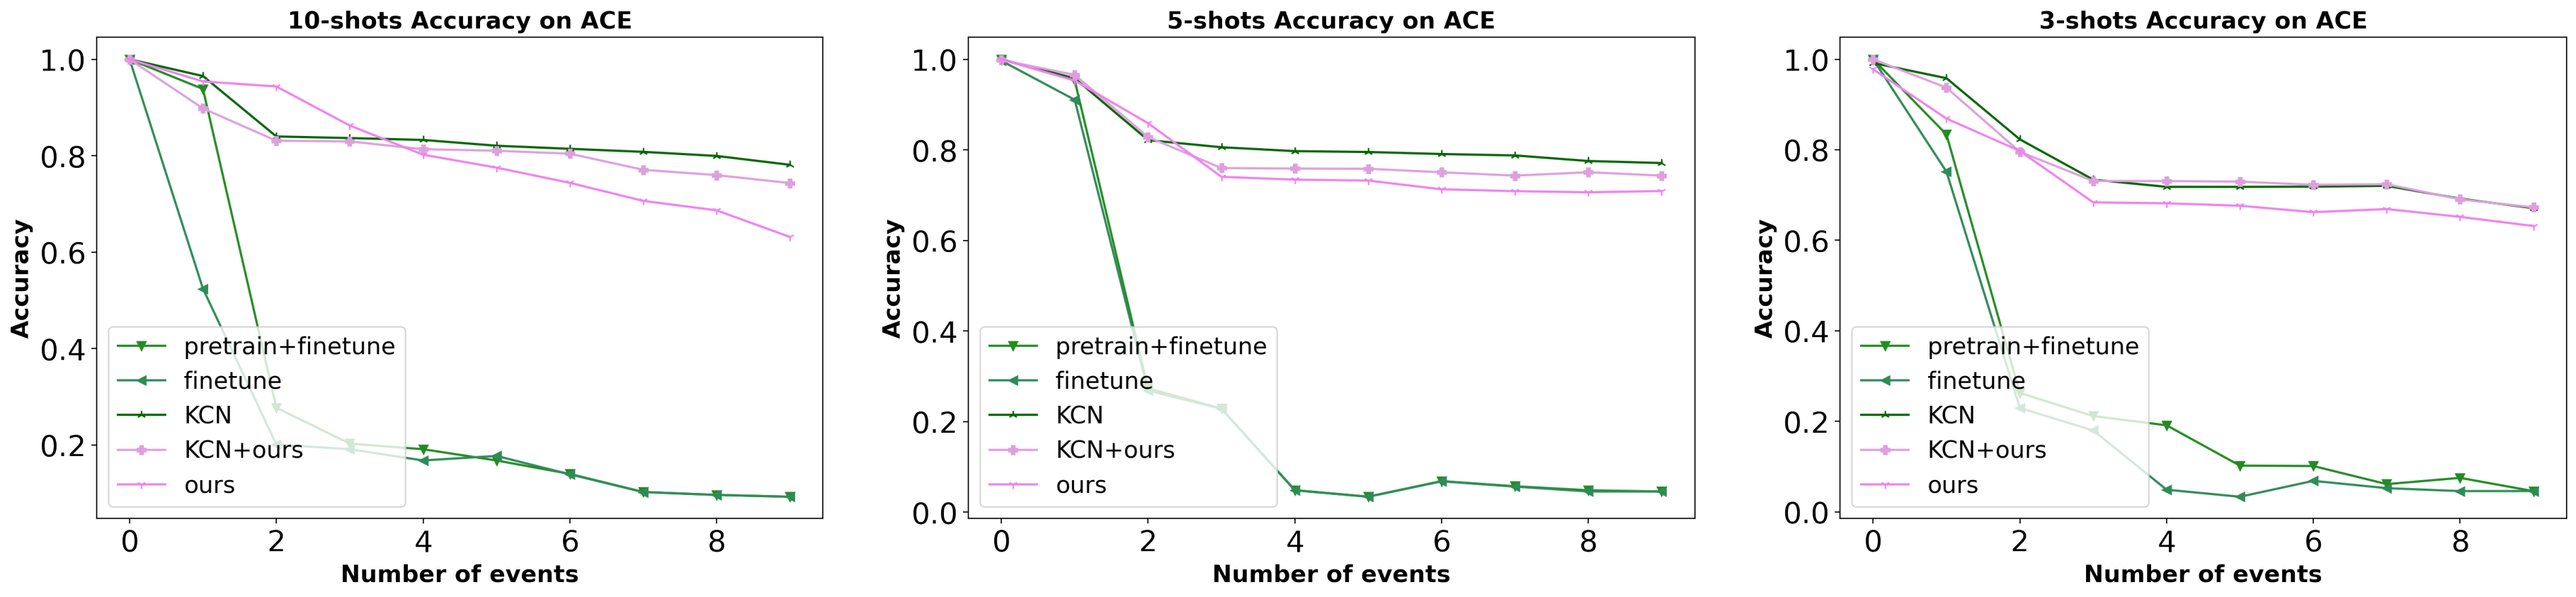
\includegraphics[width=\linewidth]{imgs/MAVEN_ACE.pdf}
%      \caption{10-shot, 5-shot, and 3-shot results using ACE05 as meta-testing set}
%      \label{fig:MAVEN_ACE}
%  \end{figure*}

\begin{figure*}[ht]
\centering
    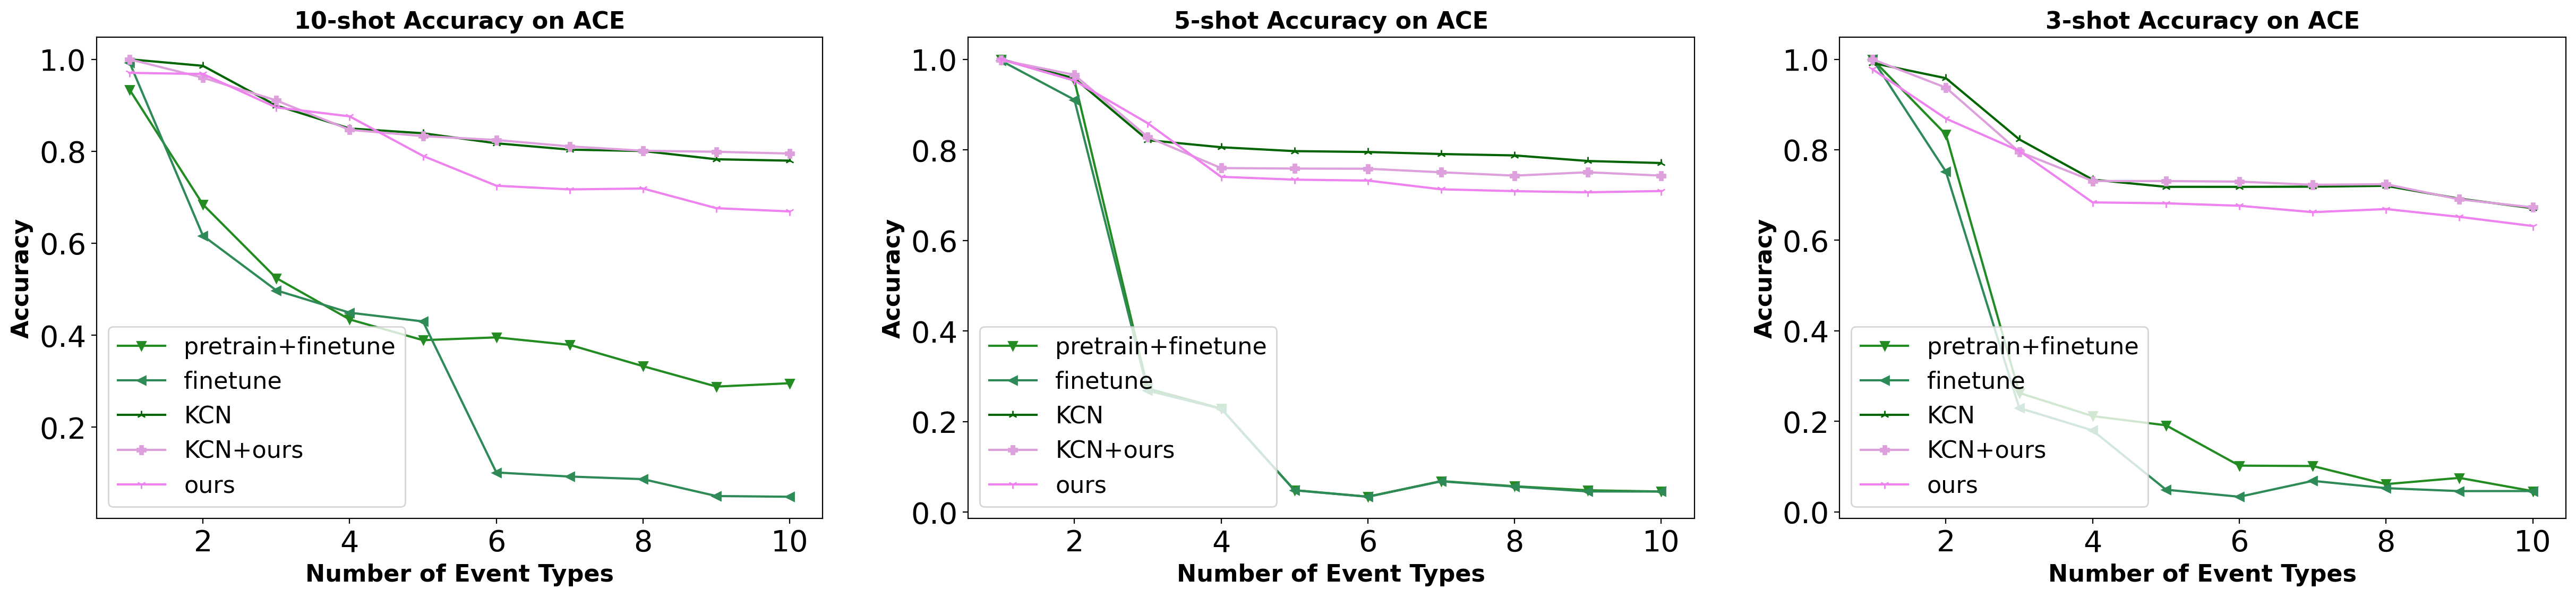
\includegraphics[scale=0.28]{imgs/MAVEN_ACE.jpg}
    \caption{10-shot, 5-shot, and 3-shot results using ACE05 as meta-testing set}
    \label{img:result_ACE}
\end{figure*}
  
\subsection{Dataset and Continual Few-shot Event Detection Task}
We adopted two widely used datasets for event detection and created the continual few-shot event detection tasks for evaluation. The dataset statistic are shown in Table~\ref{tab:stats}.

\noindent
\textbf{ACE 2005 English} \footnote{\url{https://catalog.ldc.upenn.edu/LDC2006T06}}: ACE 2005 English contains 33 event types.  To conduct our few-shot experiment, we filtered out events that have less than 10 interactions.

\noindent
\textbf{MAVEN} \citep{wang2020MAVEN}: MAVEN dataset contains 168 event types and is much more diverse compared to the ACE05 dataset. Each event types also has a significantly more instances.  Due to limited computational resources,  we choose keep the top 50 event types by number of instances.  

\noindent
\textbf{Continual Few-shot Event Detection}: There is no available benchmark for continual few-shot event detection. Therefor, we propose the following construction method: for a given dataset,  we first construct a few-shot event detection dataset following a similar setup as \citep{chen2021honey}.  In particular,  for every event type,  we subsample its instances to simulate a few-shot condition.  For each event type, we randomly sample few instances as the support set, and the all other instances are used as the query set for evaluating.  For the continual event detection,  we followed the setup in \citep{cao2020incremental}.  We exploit the data of the top 10 most frequent event classes for continual learning. One new event class will be available for the model at each time, and we test the model on all previously seen event types. 


\subsection{Meta-Training and Meta-Testing Detail}
\textbf{Meta-Training}: We used Bert \citep{devlin2018bert} as the representation module and a fully connected layer as the classifier.  In each training episode, we sample a continuous data trajectory of event instances.  The trajectory construction follows \ref{img:2}. 

\noindent
\textbf{Meta-Testing}: During the meta testing stage,  we followed the continual few-shot event detection setup. The support set for each event type comes in a class-incremental way. After each batch of support set arrives, we tested the model on all seen query sets. 

\subsection{Baselines}
We compare out approach with the following baselines: 

\noindent
\textbf{Finetune}: The model is simply fine-tuned whenever a stream of data arrives.

\noindent
\textbf{Pretrain + finetune}: We fine-tune the language model that are pretrained on the meta-training set. 

\noindent
\textbf{KCN}\citep{cao2020incremental}: KCN focuses on incremental event detection and uses prototype enhanced retrospection and hierarchical distillation to mitigate the adverse effects of semantic ambiguity and class imbalance. We initialized the language model used in KCN with a pretrained language model that is trained on the meta-training set to ensure a fair comparison. 

%We have not include the work by \cite{yu2021lifelong} 
We also implemented a model of  \cite{yu2021lifelong} following our experimental setup. However, this method could only reach an accuracy of ~0.4 while our method or KCN could reach ~0.7. There are some possible explanations for this result: 
\begin{enumerate}[noitemsep]
\item There might be some implementation errors of  \cite{yu2021lifelong} or a different configuration of hyper-parameters is required due to the new few-shots learning. For example, changing the default learning rate (1e-4)  in  \cite{yu2021lifelong}  to (6e-4) could help improve the final accuracy from ~0.1 to ~0.4. And some other hyper-parameters, i.e. the size of experience replay are also sensitive to the few-shots learning. We believe that a more concrete hyper-paramter search could further improve the performance. 

\item \cite{yu2021lifelong}  is not designed for a few-shot learning setting; there are thousands of  training data in the original experiments while there are only 10 training data in our setting. However, we believe that we could combine our model with his proposed method of knowledge distillation + knowledge transfer strategy. 

\item \cite{yu2021lifelong} adopts a different formulation of incremental event detection.
\end{enumerate}

We test our meta-learned representation for continual few-shot event detection by using it as the language model initialization for KCN. (KCN+ours), and adding a simple fully connected layer for fine-tuning(ours). 

\subsection{Experimental Setup}
While meta-testing on the ACE05 dataset, we used the MAVEN dataset as the meta-training set and vice versa.  We conducted our experiments in 10-shot, 5-shot and 3-shot settings.  We use accuracy as the evaluation metric. We choose a simple fully connected layer for the adaptation module.  All experiments were conducted on the HAL cluster \citep{HAL}. Our implementation has been submitted on Canvas. 

\subsection{Experimental Results}
As expected,  in Figure \ref{img:result_ACE} both the fine-tune and pretrain + finetune suffer from catastrophic interference. Their performance dropped significantly after 1 increment in event types. On the other hand, our meta-learned representation module with a simple fine-tune fully connected layer demonstrates strong performance across different few-shot setups.  However, it is not able to achieve the same level of performance as KCN and KCN + ours. Our speculation is that simply fine-tuning the model on the meta-learned representation module suffers from some degree of forgetting problem as it lacks the exmapler/memory set to store previous knowledge. Moreover, it cannot learn from previous examples as effectively as KCN since there is no distillation strategy. On the other hand KCN + ours outperforms KCN under the 10 shot setting, and is on par with KCN for 5-shot and 3-shot setup. 

\subsection{Case Study}
We also tested our representation module to see if it can be generalized to larger dataset.  We used ACE05 as the meta-training set and MAVEN as the meta testing set. 

\begin{figure}[h]
\centering
    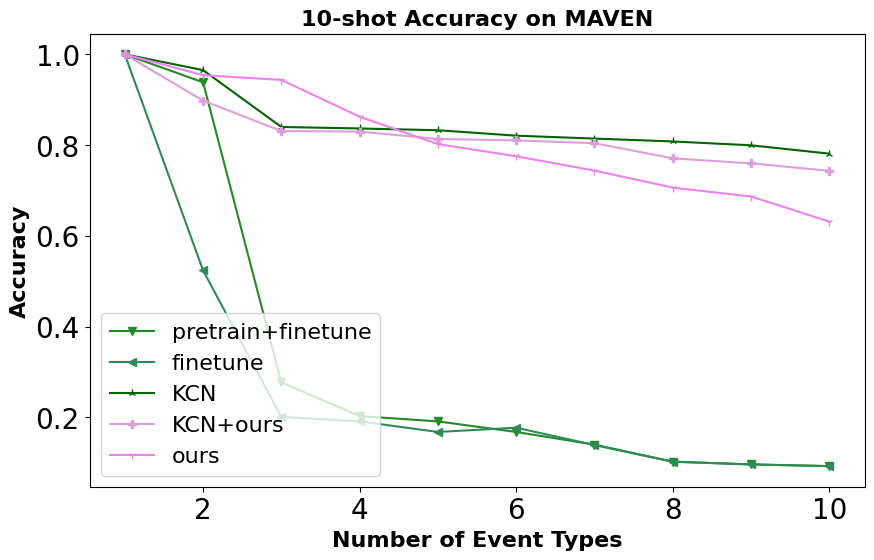
\includegraphics[scale=0.28]{imgs/ACE_MAVEN.jpg}
    \caption{10-shot results using MAVEN as meta-testing set}
    \label{img:result_MAVEN}
\end{figure}

As we can see,  both ours and KCN + ours have worse performance than KCN.  We suspect the issue is that MAVEN is a significantly larger and more diverse dataset compared to ACE05. Our meta-learned representation module might not generalize well enough to give robust performance on the continual few-shot event detection task.


\section{Related Works}
\label{sec:related_work}
\subsection{Few-shot Event Detection}
\label{sec:rw_event_detection}
Many methods have been proposed to address the few-shot event detection problem. \citet{bronstein2015seed} identify new event with feature-based method by collecting seed triggers. \citet{deng2020meta} divide the few-shot event detection into trigger extraction and few-shot classification. \citet{feng2020probing} conduct few-show classification without triggers on sentence-level. \citet{chen2021honey} using the causal intervention to address the few-shot problem.

\subsection{Continual Learning}
\label{sec:rw_continual_learning}
Much efforts have been put to study the continual learning problems. Major methods can be divided into three categories or the combination of these categories: significant parameter based methods \citep{kirkpatrick2017overcoming, aljundi2018memory}; rehearsal based methods \citep{rebuffi2017icarl, hou2019learning, shin2017continual, li2017learning, cao2020incremental}; and sparse representation methods \citep{liu2019utility, aljundi2018selfless}.
The significant parameter based methods try to recognize and reserve the significant parameters trained on old data. But it is hard to devise suitable metrics to evaluate the parameters. The rehearsal-based methods try to preserve previous knowledge via storing a few old data\citet{rebuffi2017icarl, hou2019learning}, via generative models learned on old data\citet{shin2017continual}, via knowledge distillation\citep{li2017learning}. \citep{cao2020incremental} indicates that these methods cannot
handle semantic ambiguity problem and class imbalance problem in incremental event detection. So they proposed \textit{Knowledge Consolidation Networks} based on both replay-based and knowledge distillation methods to handle these issues. However, they ignore the long-tail distribution problem \citep{yu2021lifelong}.

%\subsection{References}


%
%The \LaTeX{} and Bib\TeX{} style files provided roughly follow the American Psychological Association format.
%If your own bib file is named \texttt{custom.bib}, then placing the following before any appendices in your \LaTeX{} file will generate the references section for you:
%\begin{quote}
%\begin{verbatim}
%\bibliographystyle{acl_natbib}
%\bibliography{custom}
%\end{verbatim}
%\end{quote}



\section{Acknowledgements}

% Entries for the entire Anthology, followed by custom entries

\nocite{Ando2005,borschinger-johnson-2011-particle,andrew2007scalable,rasooli-tetrault-2015,goodman-etal-2016-noise,harper-2014-learning}
\bibliographystyle{acl_natbib}
\bibliography{custom}
\appendix

\end{document}
